%%%%%%%%%%%%%%%%%%%%%%%%%%%%%%%%%%%%%%%%%%%%%%%%%%%%%%%
% Copyright (c) 2024 Fengming Zhu. All rights reserved.
% Email:        fzhuae@connect.ust.hk
%%%%%%%%%%%%%%%%%%%%%%%%%%%%%%%%%%%%%%%%%%%%%%%%%%%%%%%


\documentclass{beamer}
\usepackage{hyperref}
\usepackage[T1]{fontenc}
\usepackage[numbers]{natbib}
%\UseRawInputEncoding

\usetheme{metropolis}
\definecolor{white}{rgb}{1,1,1}
\beamersetaveragebackground{white}

% other packages
\usepackage{latexsym,amsmath,xcolor,multicol,booktabs,calligra}
\usepackage{amsfonts, amssymb}
\usepackage{graphicx,listings,stackengine}
\usepackage{ulem}

% \usepackage[loadonly]{enumitem}
% \setlistdepth{20}
% \renewlist{itemize}{itemize}{20}

%% Enable only in Xelatex
% \usepackage{pstricks}

\author{Fengming ZHU}  % you can change it to your name
\title{COMP3211 Tutorial 6: MDP/RL}
\institute{Department of CSE \\ HKUST \\ {\copyright\ 2024 Fengming Zhu. All rights reserved.}}
\date{Apr. 15\&18, 2024} % you can change it to the latest date


% defs
\def\cmd#1{\texttt{\color{red}\footnotesize $\backslash$#1}}
\def\env#1{\texttt{\color{blue}\footnotesize #1}}
\definecolor{deepblue}{rgb}{0,0,0.5}
\definecolor{deepred}{rgb}{0.6,0,0}
\definecolor{deepgreen}{rgb}{0,0.5,0}
\definecolor{halfgray}{gray}{0.55}

\lstset{
    basicstyle=\ttfamily\small,
    keywordstyle=\bfseries\color{deepblue},
    emphstyle=\ttfamily\color{deepred},    % Custom highlighting style
    stringstyle=\color{deepgreen},
    numbers=left,
    numberstyle=\small\color{halfgray},
    rulesepcolor=\color{red!20!green!20!blue!20},
    frame=shadowbox,
}

{}
\begin{document}

\begin{frame}
    \titlepage
\end{frame}


% \begin{frame}{References}
% \begin{itemize}
%     \item \underline{Main focus}
%     \begin{itemize}
%         \item
%         (SoCS'2013) \textbf{Multi-Agent Path Finding for Self Interested Agents}
%         \cite{bnaya2013multi}
        
%         \item
%         (AAAI'2015) \textbf{Multi-Agent Pathfinding as a Combinatorial Auction}
%         \cite{amir2015multi}

%         \item
%         (Tech report) \textbf{An Empirical Evaluation of a Combinatorial Auction for Solving Multi-Agent Pathfinding Problems}
%     \end{itemize}

%     \item Related
%     \begin{itemize}
%         \item
%         (AAMAS'2019) \textit{Polynomial-Time Multi-Agent Pathfinding with Heterogeneous and Self-Interested Agents}
%         \cite{machida2019polynomial}

%         \item
%         (IROS'2020) \textit{Path Negotiation for Self-interested Multirobot Vehicles in Shared Space}
%         \cite{inotsume2020path}
%     \end{itemize}
% \end{itemize}
% \end{frame}


\begin{frame}{Outline}
    % \tableofcontents[sectionstyle=show,subsectionstyle=show/shaded/hide,subsubsectionstyle=show/shaded/hide]
    \tableofcontents[
    sectionstyle=show,
    subsectionstyle=shaded,
    subsubsectionstyle=shaded
    ]
\end{frame}


\section{MDP V.S. Search}


\begin{frame}{MDP V.S. Search}
    \begin{exampleblock}{Search:}
        \begin{itemize}
            \item A set of states $\mathcal{S}$, initial state $I$, goal state $G$

            \item A set of actions $\mathcal{A}$

            \item Deterministic transitions $T: \mathcal{S} \times \mathcal{A} \mapsto \mathcal{S}$

            \item cost function $c: \mathcal{S} \times \mathcal{A} \mapsto \mathbb{R}$

            \item Objective: a path $p$ from $I$ to $G$ that minimizes $c(p)$
        \end{itemize}
    \end{exampleblock}

    \pause
    \vspace{-3mm}
    \begin{exampleblock}{MDP:}
        \begin{itemize}
            \item A set of states $\mathcal{S}$, a terminating condition $End(s)$

            \item A set of actions $\mathcal{A}$

            \item Stochastic transitions $T: \mathcal{S} \times \mathcal{A} \mapsto \Delta(\mathcal{S})$

            \item Reward function $r: \mathcal{S} \times \mathcal{A} \times \mathcal{S} \mapsto \mathbb{R}$, with a discount factor $\gamma$

            \item Objective: maximize $\sum_t \gamma^t r_t$
        \end{itemize}
    \end{exampleblock}
\end{frame}

\begin{frame}{Solution Concept: Policy}
    \begin{exampleblock}{Question:}
        Given a sequential and stochastic decision making problem, in order to come up with an optimal solution, you'd like to know:
        \begin{itemize}
            \item (A) Only your current state

            \item (B) All the history from the beginning up until now

            \item (C) Need to know more
        \end{itemize}
    \end{exampleblock}

    \pause
    \begin{exampleblock}{Markov property:}
        A state $S_t$ is Markovian iff $P[S_{t+1}| S_{t}, \cdots, S_0] = P[S_{t+1}| S_{t}]$.
        That is, your current state is already a ``sufficient statistic'' that well summarizes the history,
        also known as the \alert{information state}.
    \end{exampleblock}

    \pause
    \begin{exampleblock}{Policy in MDP:}
        A solution is a policy $\pi: \mathcal{S} \rightarrow \Delta(\mathcal{A})$ 
    \end{exampleblock}

\end{frame}

\begin{frame}{Follow-up Question: Maze}
    \begin{exampleblock}{Question:}
        Given a large maze,
        you (with deterministic actions U/D/L/R) are supposed to find a nice way from the entrance to the exit,
        which agent you'd like to choose
        \begin{itemize}
            \item (A) State machines with infite memory
            \item (B) Agents that can do $A^*$ search
            \item (C) Agents that can compute policies
            \item (D) None of them
        \end{itemize}
        
        \vspace{-3mm}
        \begin{figure}[htpb]
            \centering
            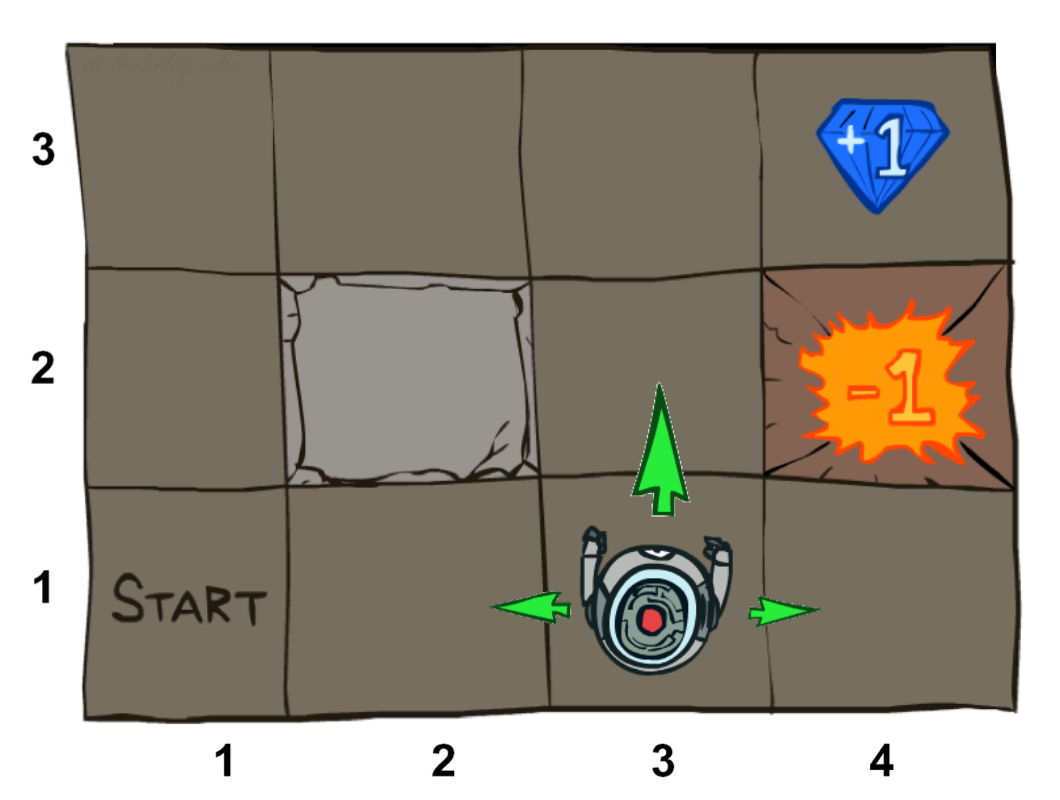
\includegraphics[width=0.3\linewidth]{pic/maze.png}
            \pause
            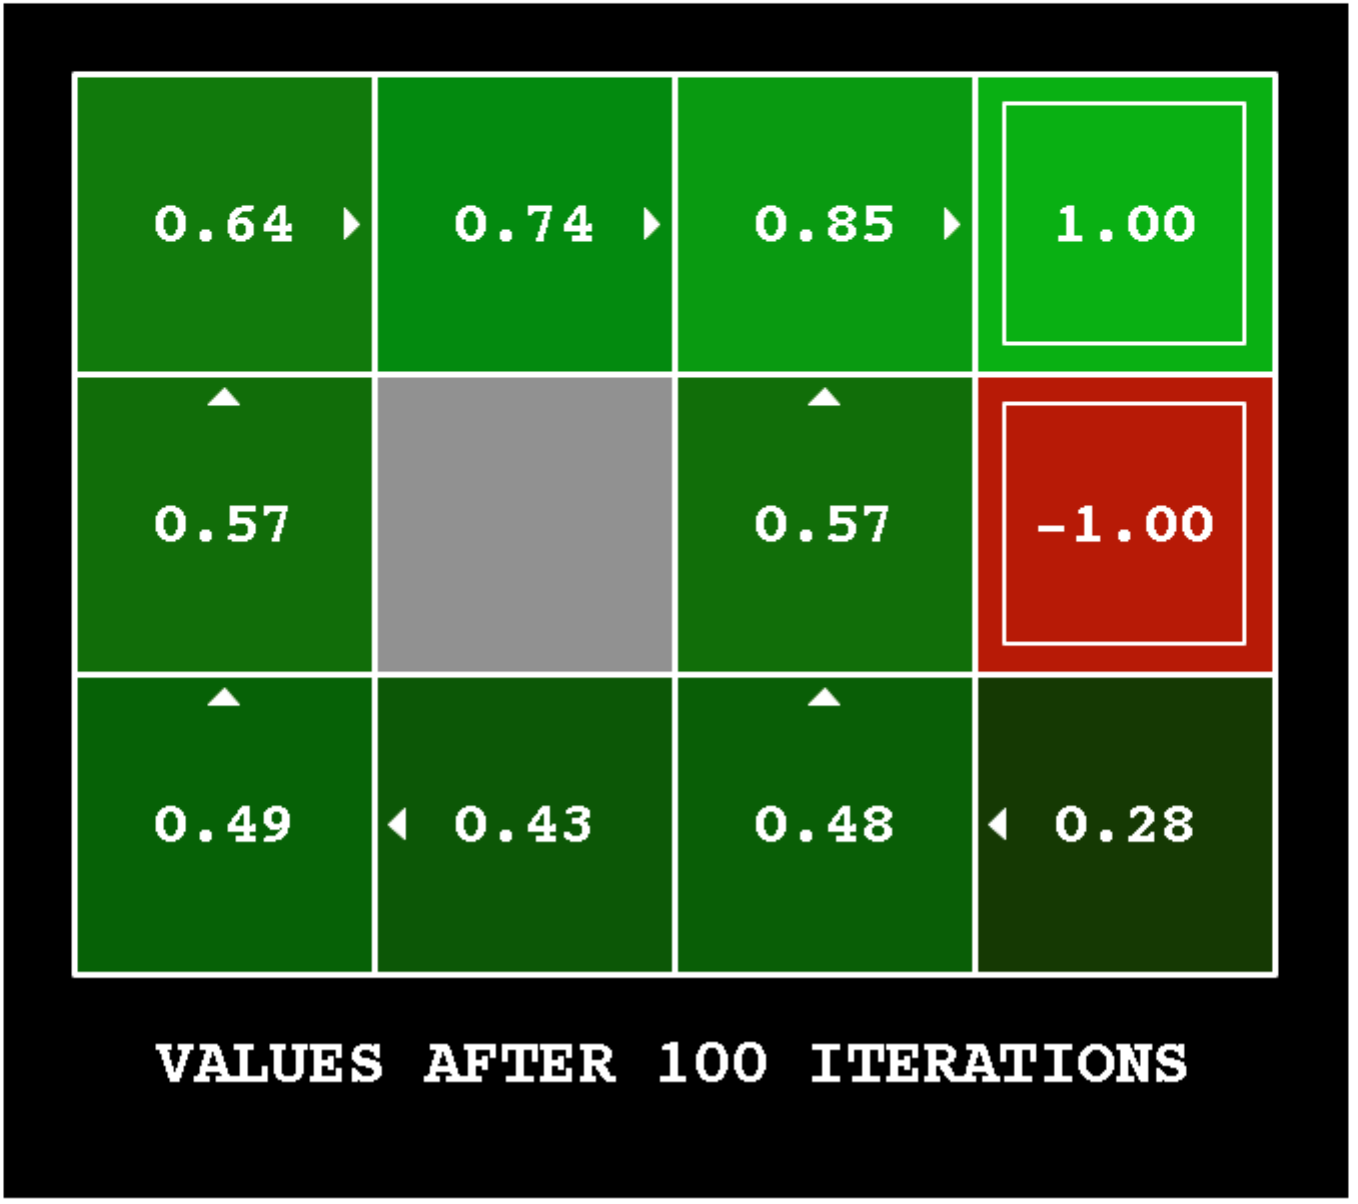
\includegraphics[width=0.25\linewidth]{pic/maze_ret.png}
        \end{figure}
    \end{exampleblock}
\end{frame}


\begin{frame}{Tree Search: A Conceptual Bridge}
\begin{figure}[htpb]
\centering
    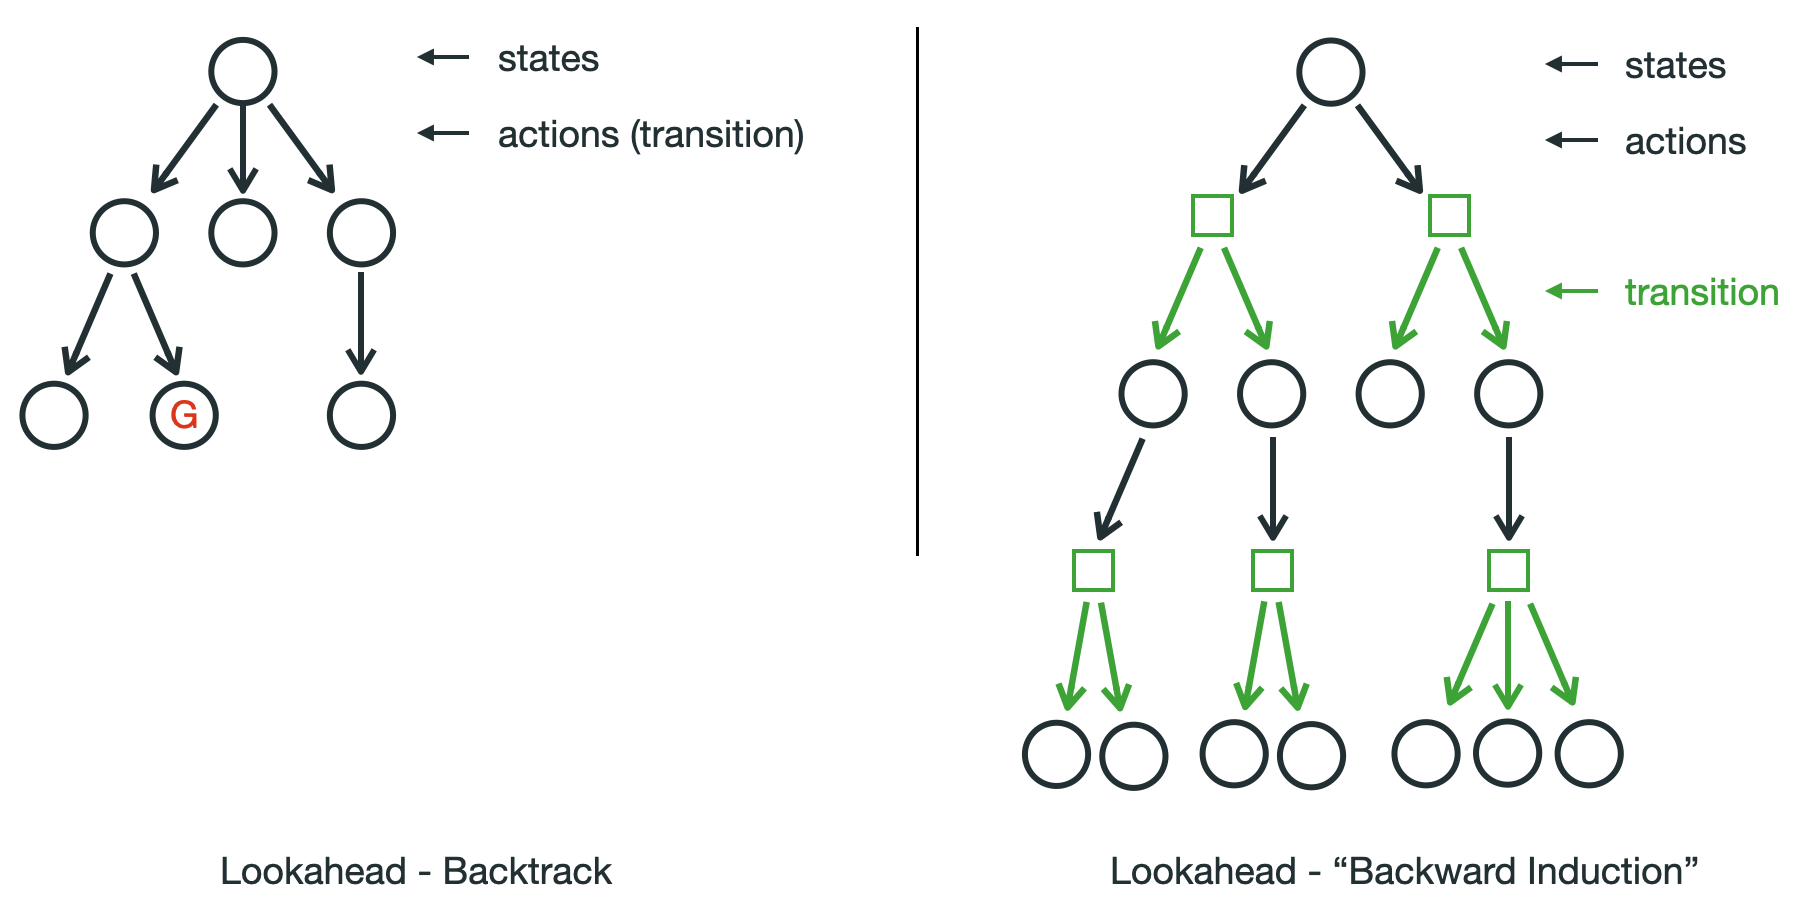
\includegraphics[width=1\linewidth]{pic/tree.png}
\end{figure}
\centering
\alert{A policy is nothing but a conditional plan!}

\pause
\alert{What if (1) repeat states; (2) infinite horizon?}
\end{frame}


\begin{frame}{Bellman (Optimality) Equation}
    \begin{itemize}
        \item For state-value function,
        \[
        v_*(s) = \max_a \sum_{s'\in S} T(s, a, s')[R(s, a, s') + \gamma v_*(s')]
        \]
        
        \item For action-value function,
        \[
        q_*(s,a) 
        = \max_a \sum_{s'\in S} T(s, a, s')[R(s, a, s') + \gamma \max_{a'} q_*(s', a')]
        \]
        \item \alert{However, non-linear thus no closed form solution in general!}
    \end{itemize}
\end{frame}


\section{Policy Iteration/Value Iteration}



\begin{frame}{Policy Interation}
    \begin{exampleblock}{Policy iteration:}
  	\begin{itemize}
  		\item Initialize $\pi \gets \pi_0, v(\cdot) \gets \vec{0}$
  		\item While $\pi$ still changing:
  		\begin{itemize}
  			\item \underline{Policy evaluation}: iterate \textbf{until convergence}
  			$\forall s,
  			v^t_\pi(s) \gets \sum_a \pi(a|s)\cdot \sum_{s'\in S} T(s, a, s')[R(s, a, s') + \gamma v^{t-1}_\pi(s')]$
  			\item \underline{Policy improvement}: greedy update
			$\forall s,
			\pi_{+}(s) \gets \arg\max_{a\in A(s)} q_{\pi}(s, a)$
  			\item $\pi \gets \pi_{+}$
  		\end{itemize}
  	\end{itemize}
    \end{exampleblock}
\end{frame}


\begin{frame}{Value Interation}
    \begin{exampleblock}{Value iteration:}
  	\begin{itemize}
  		\item Initialize $\pi \gets \pi_0, v(\cdot) \gets \vec{0}$
  		\item While $V$ still changing:
  		\[
  		\forall s,
  		v_*^{t+1}(s)
  		\gets \max_a \sum_{s'\in S} T(s, a, s')[R(s, a, s') + \gamma v_*^t(s')]
  		\]
  		\item Extract $\pi_*$
  		\[
  		\forall s, \pi_*(s) \gets \arg\max_a \sum_{s'\in S} T(s, a, s')[R(s, a, s') + \gamma v_*(s')]
  		\]
  	\end{itemize}
    \end{exampleblock}
    
\alert{But note that, intermediate value functions might not correspond to any underlying policy $\pi$.}
\end{frame}

\begin{frame}{Value Interation}
    \begin{exampleblock}{Value iteration (another perspective):}
  	\begin{itemize}
  		\item Initialize $\pi \gets \pi_0, v(\cdot) \gets \vec{0}$
  		\item While $V$ still changing:
  		\begin{itemize}
  			\item \underline{Policy evaluation (one sweep)}: iterate \textbf{only once}
  			$\forall s,
  			v(s) \gets \sum_a \pi(a|s)\sum_{s'\in S} T(s, a, s')[R(s, a, s') + \gamma v(s')]$
  			\item \underline{Policy improvement}: greedy update
			$\forall s,
			\pi_{+}(s) \gets \arg\max_{a\in A(s)} q(s, a)$
			
  			\item $\pi \gets \pi_{+}$ (every $\pi$ will be deterministic except for $\pi_0$)
  		\end{itemize}
  	\end{itemize}
    \end{exampleblock}
\alert{Still, intermediate value functions might not correspond to any underlying policy $\pi$.}
\end{frame}

\begin{frame}{REINFORCEjs: Dynamic Programming Demo}
\begin{figure}[htpb]
    \centering
    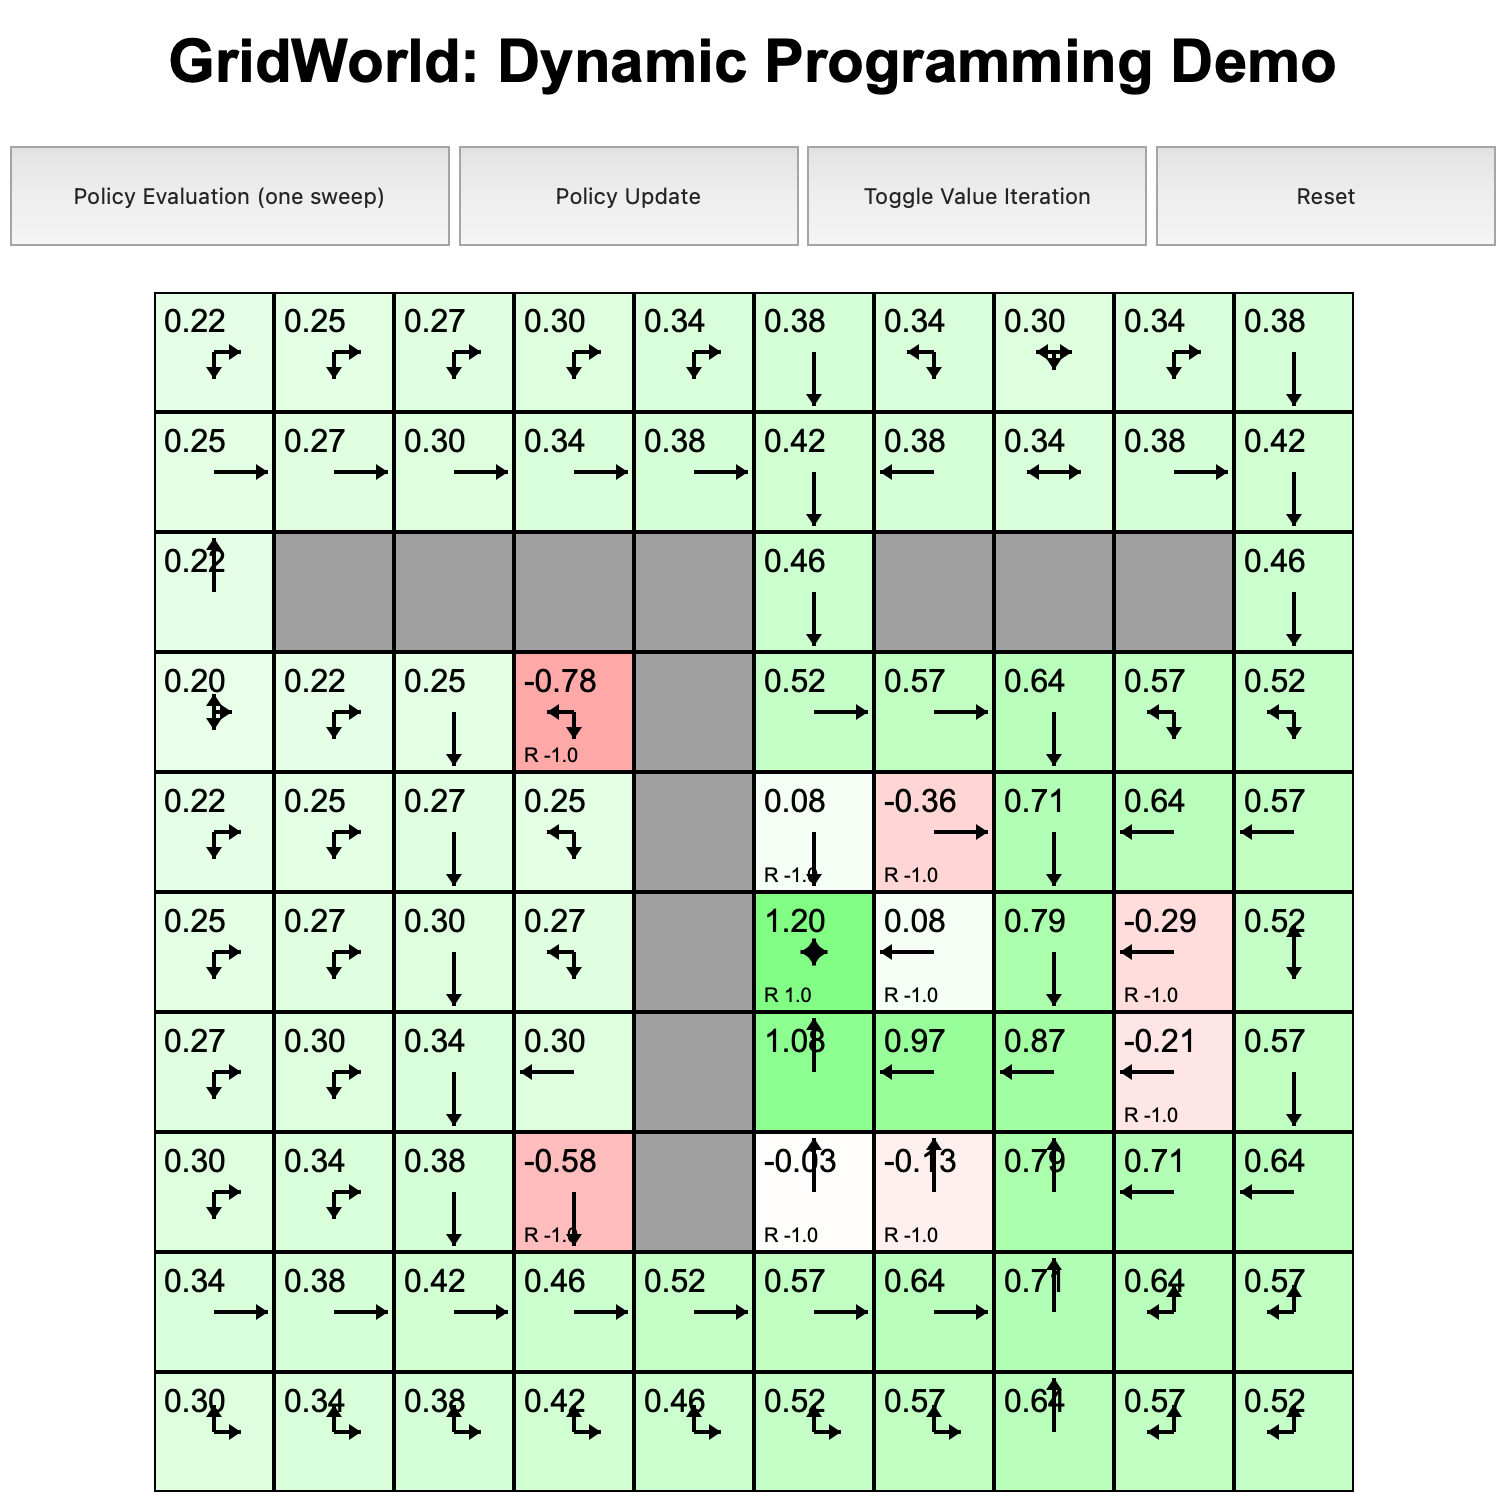
\includegraphics[width=0.6\linewidth]{pic/jsgrid.png}
    \tiny{https://cs.stanford.edu/people/karpathy/reinforcejs/gridworld\_dp.html}
\end{figure}
\end{frame}
%
%\subsection{A Toy Example: Golf Play}
%
%\begin{frame}{A Toy Example: Golf Play}
%\vspace{-0mm}
%\begin{figure}[htpb]
%    \centering
%    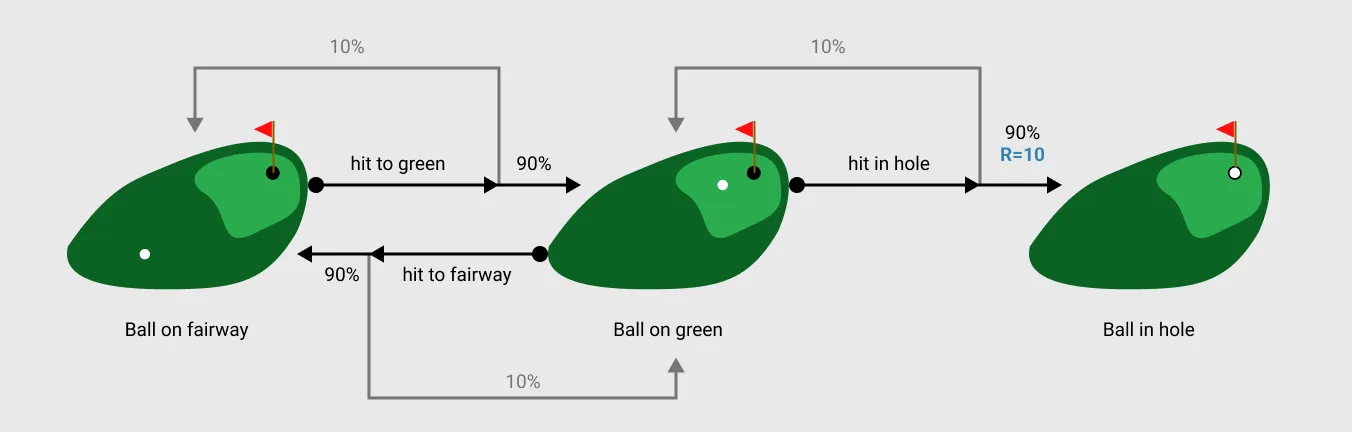
\includegraphics[width=0.7\linewidth]{pic/golf.png}
%\end{figure}
%
%\vspace{-2mm}
%\begin{exampleblock}{MDP formulation:}
%	\begin{itemize}
%		\item $S = \{s_0, s_1, s_2\}$
%		\item $A = \{hg, hf, hh\}$
%		\item Transitions: $T(s_1|s_0, hg) = 0.9, T(s_0|s_0, hg) = 0.1$, $T(s_2|s_1, hh) = 0.9, T(s_1|s_1, hh) = 0.1$, $T(s_0|s_1, hf) = 0.9, T(s_1|s_1, hf) = 0.1$.
%		\item Rewards: $R(s_1, hh, s_2) = 10$, otherwise 0.
%		\item $\gamma = 0.9$
%
%	\end{itemize}
%\end{exampleblock}
%\end{frame}
%
%
%\begin{frame}{A Toy Example: Golf Play - policy iteration}
%\begin{enumerate}
%	\item [0.] $\pi_0 \gets uniform, V(\cdot) \gets all\ zeros$
%	\begin{enumerate}
%		\item $V^1(s_0) = T(s_1|s_0, hg) * [\gamma V^0(s_1) + R(s_0, hg, s_1)] + \ T(s_0|s_0, hg) * [\gamma V^0(s_0) + R(s_0, hg, s_0)]$
%		
%	\end{enumerate}
%\end{enumerate}
%\end{frame}
%
%
%\begin{frame}{A Toy Example: Golf Play - value iteration}
%
%\end{frame}


\section{Coding Examples}

\subsection{Grid Worlds - via Policy Iteration}

\begin{frame}{$3 \times 3$ Grid World}
\begin{figure}[htpb]
    \centering
    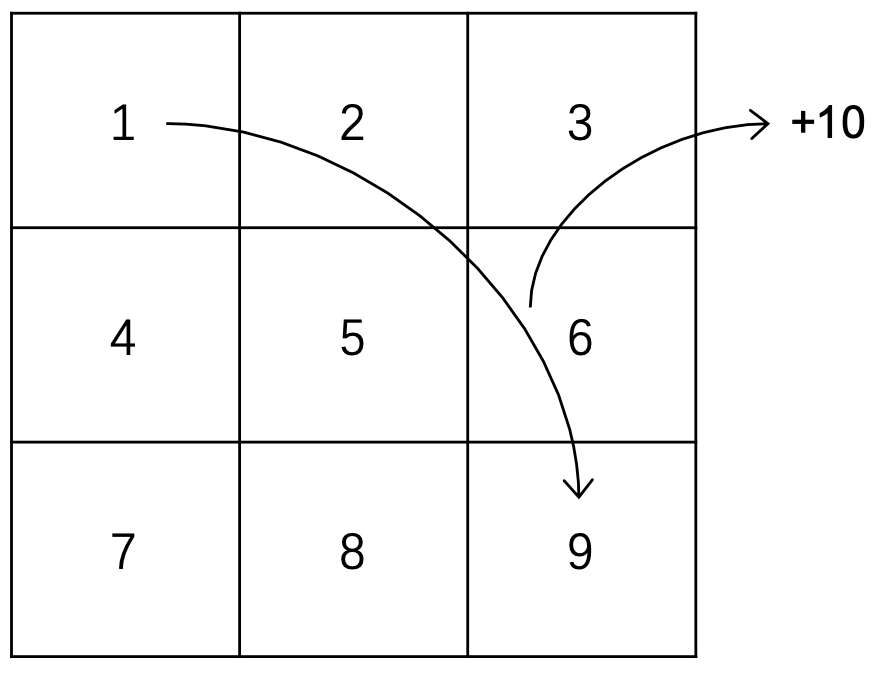
\includegraphics[width=0.4\linewidth]{pic/33grid.png}
\end{figure}

The agent can be in one of the nine cells at any starting time. It can then move in one of four directions: \{E,S,W,N\}. If the agent hits a wall, it remains in its current cell and gets a reward 1. When the agent moves to cell 1, it then immediately moves to cell 9 and gets a reward of 10. The discount factor $\gamma = 0.9$.
\end{frame}

\begin{frame}{Evaluate the uniform policy - Iterative procedures}
\begin{figure}[htpb]
    \centering
    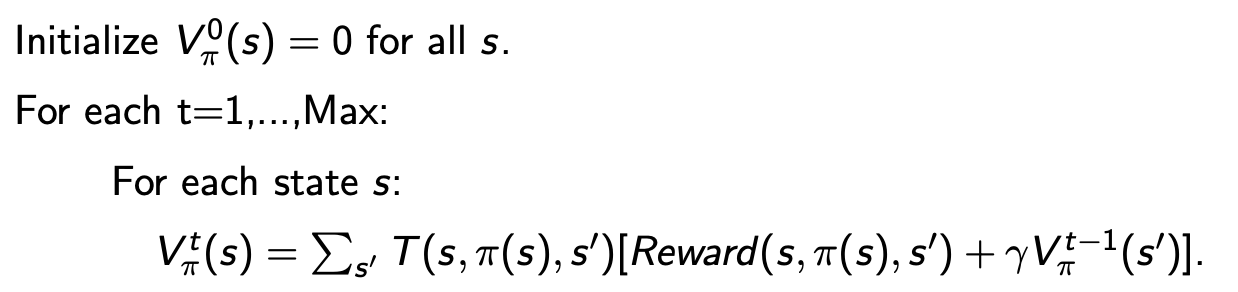
\includegraphics[width=0.8\linewidth]{pic/iterative.png}
\end{figure}

\begin{figure}[htpb]
    \centering
    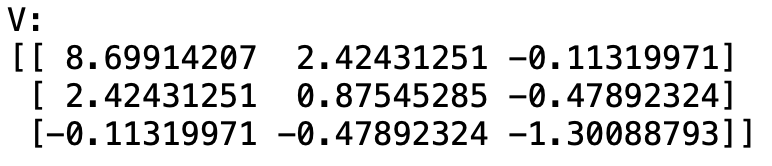
\includegraphics[width=0.7\linewidth]{pic/iterative_v.png}
\end{figure}
\end{frame}


\begin{frame}{Evaluate the uniform policy - Matrix form}
\begin{figure}[htpb]
    \centering
    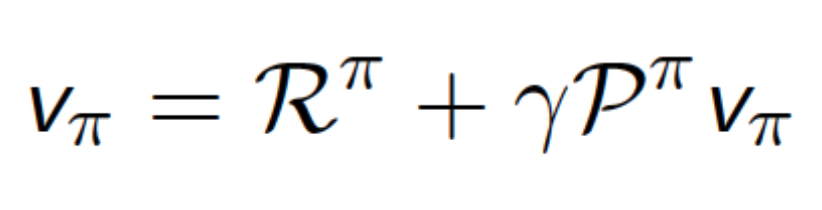
\includegraphics[width=0.4\linewidth]{pic/matrix.png}
    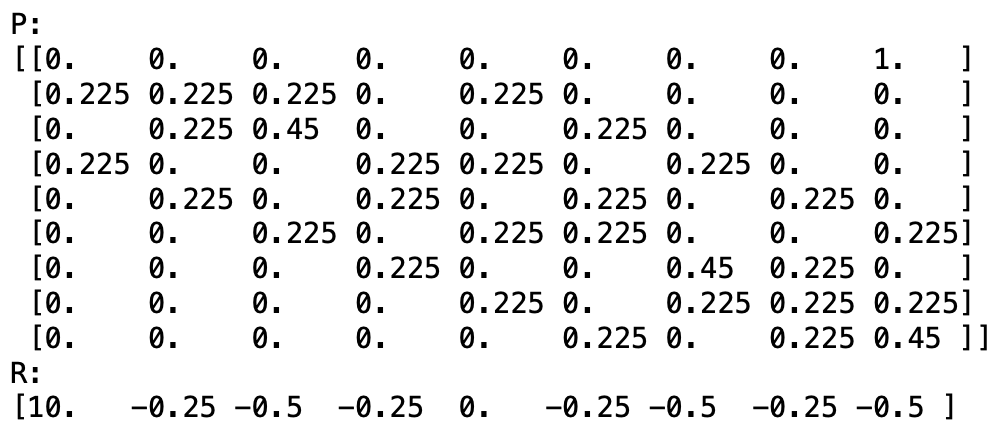
\includegraphics[width=0.8\linewidth]{pic/PR.png}
\end{figure}

\begin{figure}[htpb]
    \centering
    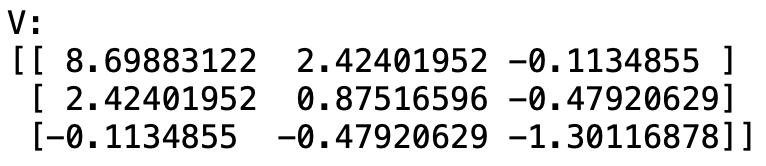
\includegraphics[width=0.7\linewidth]{pic/matrix_v.png}
\end{figure}
\end{frame}


\begin{frame}{Find the optimal policy - Analytically}
Analytically, the optimal policy for every state is to get state 1 as soon as possible. For state 9, the minimal number of steps to reach state 1 is 4 and then agent jumps back to state 9. Thus,
\[
V_1 = V_9 + 10, V_9 = 0.9^4 V_1
\Rightarrow 
V_1 = 29.08, V_9 = 19.08
\]  
The value of rest states are
$$V_2 = 0.9 V_1 = 26.17, V_3 = 0.9 V_2 = 23.55, V_4 = 0.9 V_1 = 26.17,$$
$$V_5 = 0.9 V_2 = 23.55, V_6 = 0.9 V_3 = 21.20, V_7 = 0.9 V_4 = 23.55,$$
$$V_8 = 0.9 V_7 = 21.20$$

The optimal policy will be 
\[
\begin{tabular}{|c|c|c|}
\hline
 NULL & $\leftarrow$ & $\leftarrow$ \\
\hline
 $\uparrow$ & $\leftarrow \uparrow$ & $\leftarrow \uparrow$ \\
\hline 
 $\uparrow$ & $\leftarrow \uparrow$ & $\leftarrow \uparrow$ \\
\hline
\end{tabular}
\]    
\end{frame}

\begin{frame}{Find the optimal policy - Policy iteration}
See \texttt{mdp\_example.ipynb}

Optimal state-values:
\begin{figure}[htpb]
    \centering
    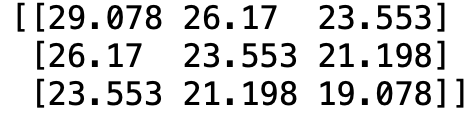
\includegraphics[width=0.5\linewidth]{pic/policy_iter.png}
\end{figure}

Extracted policy (random tie-breaking):
\[
\begin{tabular}{|c|c|c|}
\hline
 NULL & $\leftarrow$ & $\leftarrow$ \\
\hline
 $\uparrow$ & $\leftarrow $ & $\leftarrow $ \\
\hline 
 $\uparrow$ & $\leftarrow $ & $\leftarrow $ \\
\hline
\end{tabular}
\] 
\end{frame}




\subsection{Gambler's Problem - via Value Iteration}
\begin{frame}{Gambler's Problem}
(Sutton's book, example 4.3)

A gambler has the opportunity to make bets on the outcomes of a sequence of coin flips.
If the coin comes up heads, he wins as many dollars as he has staked on that flip; if it lands with tails, he loses his stake. 
The game ends when the gambler wins by reaching his goal of \$100, or loses by running out of money. On each flip, the gambler must decide what portion of his capital to stake, in integer numbers of dollars. 
\end{frame}

\begin{frame}{Gambler's Problem- Formulation}
This problem can be formulated as an undiscounted, episodic, finite MDP. The state is the gambler's capital, $s \in \{1,2,...,99\}$and the actions are stakes, $a \in \{0,1,..., \min(s,100-s)\}$. 
The reward is zero on all transitions except those on which the gambler reaches his goal, when it is +1. 
The state-value function then gives the probability of winning from each state. A policy is a mapping from levels of capital to stakes. 
The optimal policy maximizes the probability of reaching the goal. 
Let $p_h$ denote the probability of the coin coming up heads. 
If $p_h$ is known, then the entire problem is known and it can be solved, for instance, by value iteration. 
\end{frame}

\begin{frame}{Gambler's Problem - Value iteration}
    See \texttt{mdp\_example.ipynb}
\end{frame}

\begin{frame}{Gambler's Problem - Results}
\begin{figure}[htpb]
    \centering
    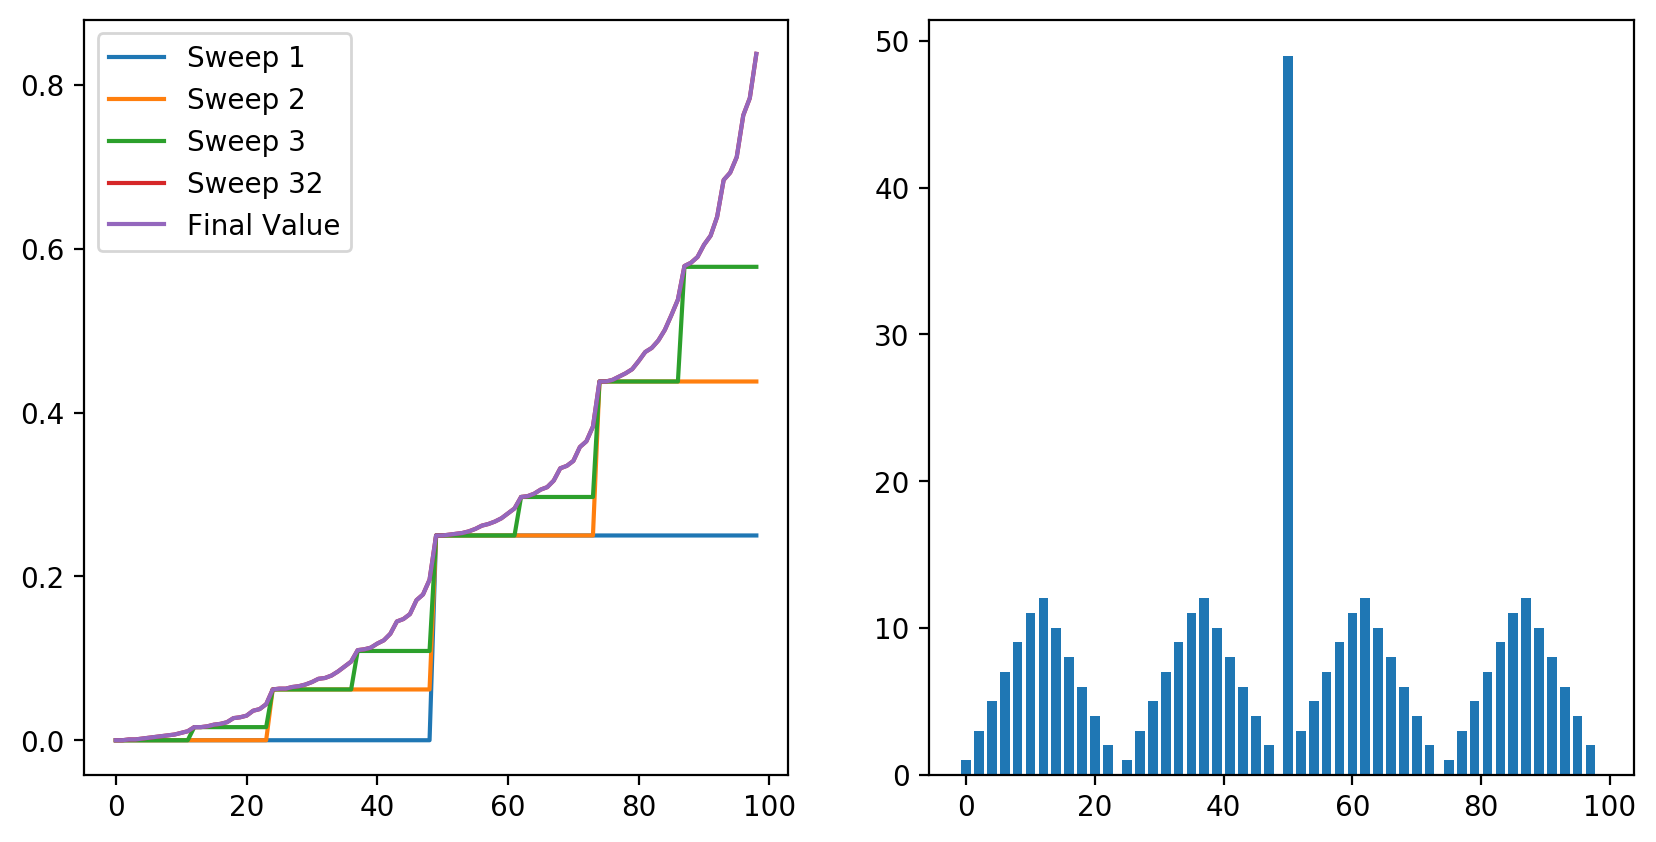
\includegraphics[width=0.6\linewidth]{pic/gambler25.png}
    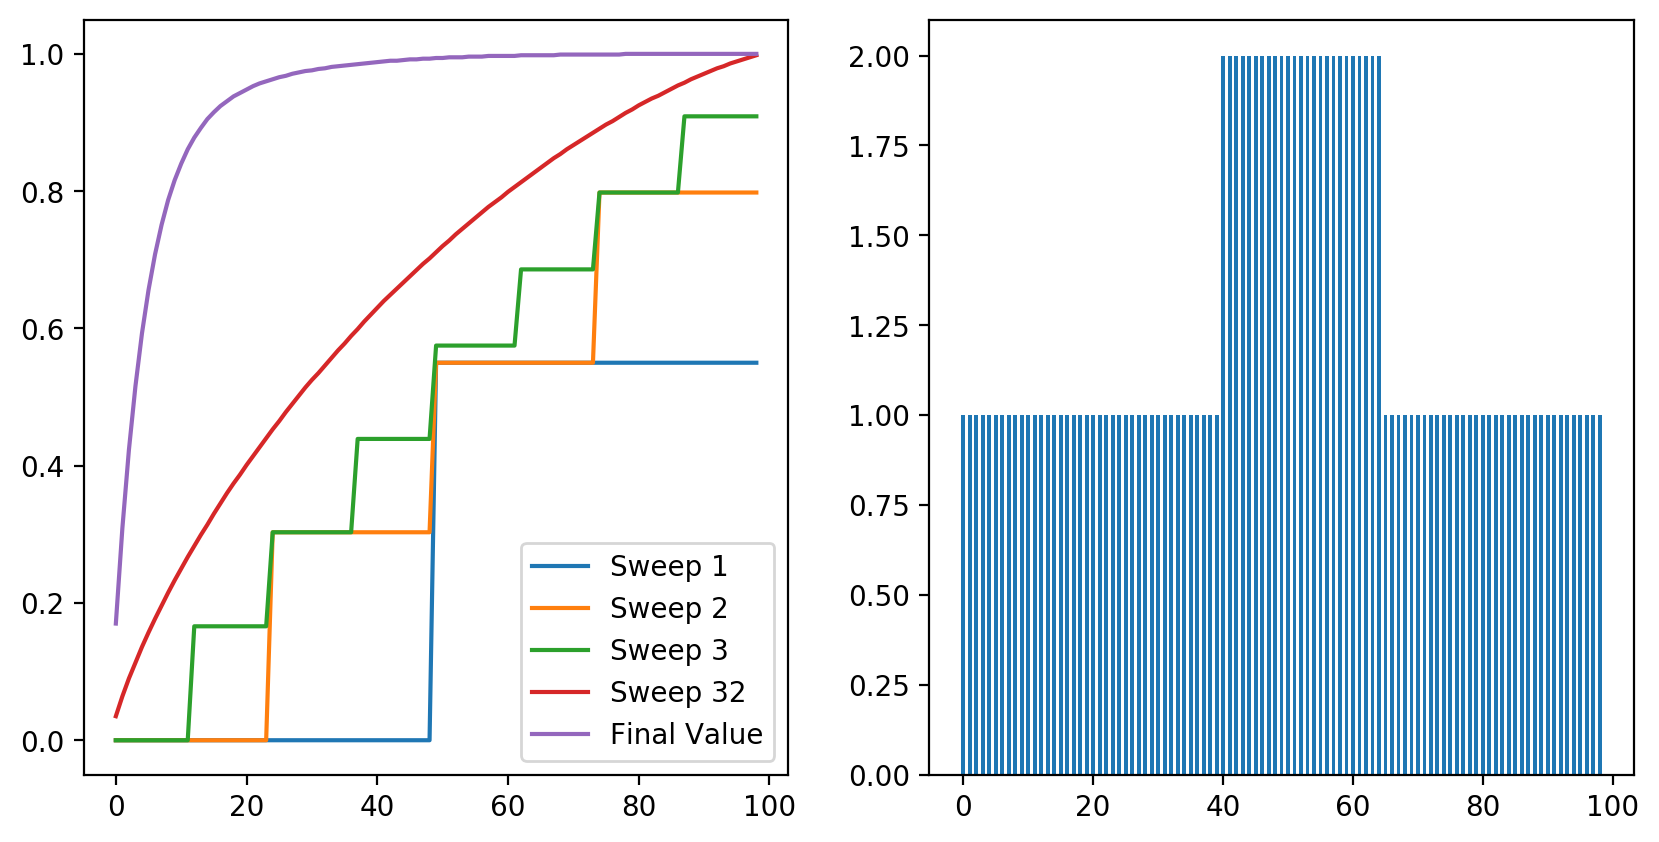
\includegraphics[width=0.6\linewidth]{pic/gambler55.png}
    \caption{$p_h=0.25 (top), p_h=0.55 (bottom)$}
\end{figure}
\end{frame}


\subsection{Maximization Bias Problem - via Q Learning}
\begin{frame}{Maximization Bias Problem}
(Sutton's book, example 6.7)

Consider a single state s where there are many actions a whose true values, q(s,a), are all zero but whose estimated values, Q(s,a), are uncertain and thus distributed some above and some below zero. The maximum of the true values is zero, but the maximum of the estimates is positive, a positive bias. We call this maximization bias.
\end{frame}

\begin{frame}{Maximization Bias Problem}
\begin{figure}[htpb]
    \centering
    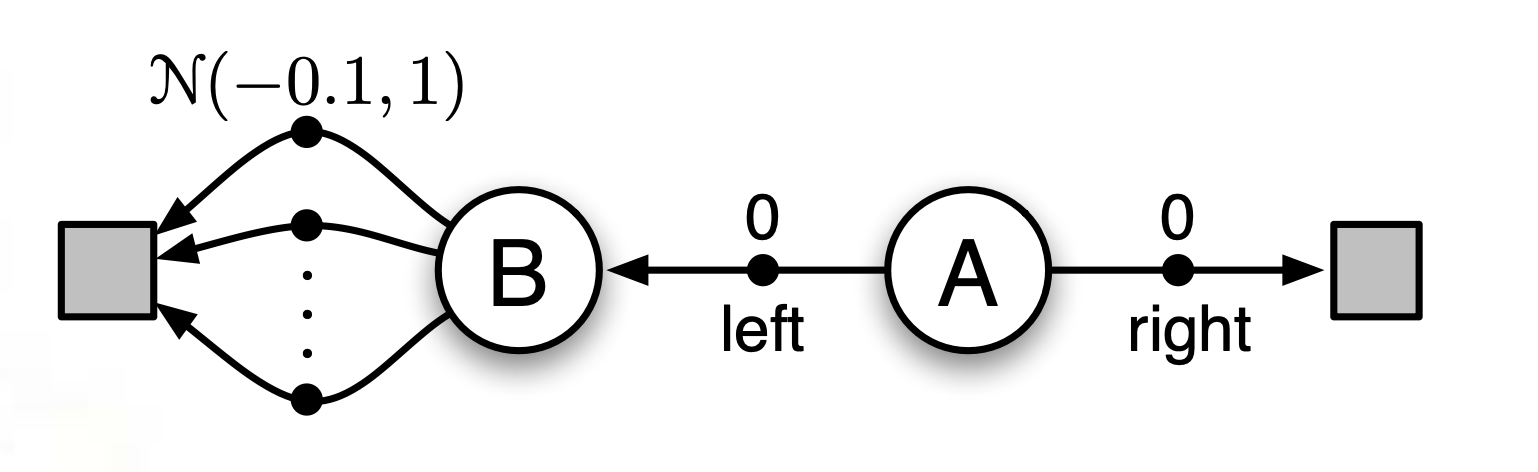
\includegraphics[width=0.7\linewidth]{pic/max_bias.png}
    \caption{Example for maximization bias.}
\end{figure}
The MDP has two non-terminal states A and B. Episodes always start in A with a choice between two actions, left and right. The right action transitions immediately to the terminal state with a reward and return of zero. The left action transitions to B, also with a reward of zero, from which there are many possible actions all of which cause immediate termination with a reward drawn from a normal distribution with mean 0.1 and variance 1.0.
\end{frame}


\begin{frame}{Maximization Bias Problem - Q Learning}
While observing (S, A, R, S')... 
\begin{exampleblock}{Q Learning}
$\epsilon$-greedy according to Q and update it\\
$
Q(S,A)
\gets (1-\alpha)Q(S,A)
+ \alpha(R + \gamma \max_{a\in A}Q(S',a)) 
$
\end{exampleblock}

\begin{exampleblock}{Double Q Learning}
$\epsilon$-greedy according to $Q_1+Q_2$ and update them\\
$
Q_1(S,A)
\gets (1-\alpha)Q_1(S,A)
+ \alpha(R + \gamma Q_2(S', \arg\max_{a\in A} Q_1(S',a)))
$
$
Q_2(S,A)
\gets (1-\alpha)Q_2(S,A)
+ \alpha(R + \gamma Q_1(S', \arg\max_{a\in A} Q_2(S',a)))
$
\end{exampleblock}

See \texttt{mdp\_example.ipynb}
\end{frame}

\begin{frame}{Maximization Bias Problem - Results}
\begin{figure}[htpb]
    \centering
    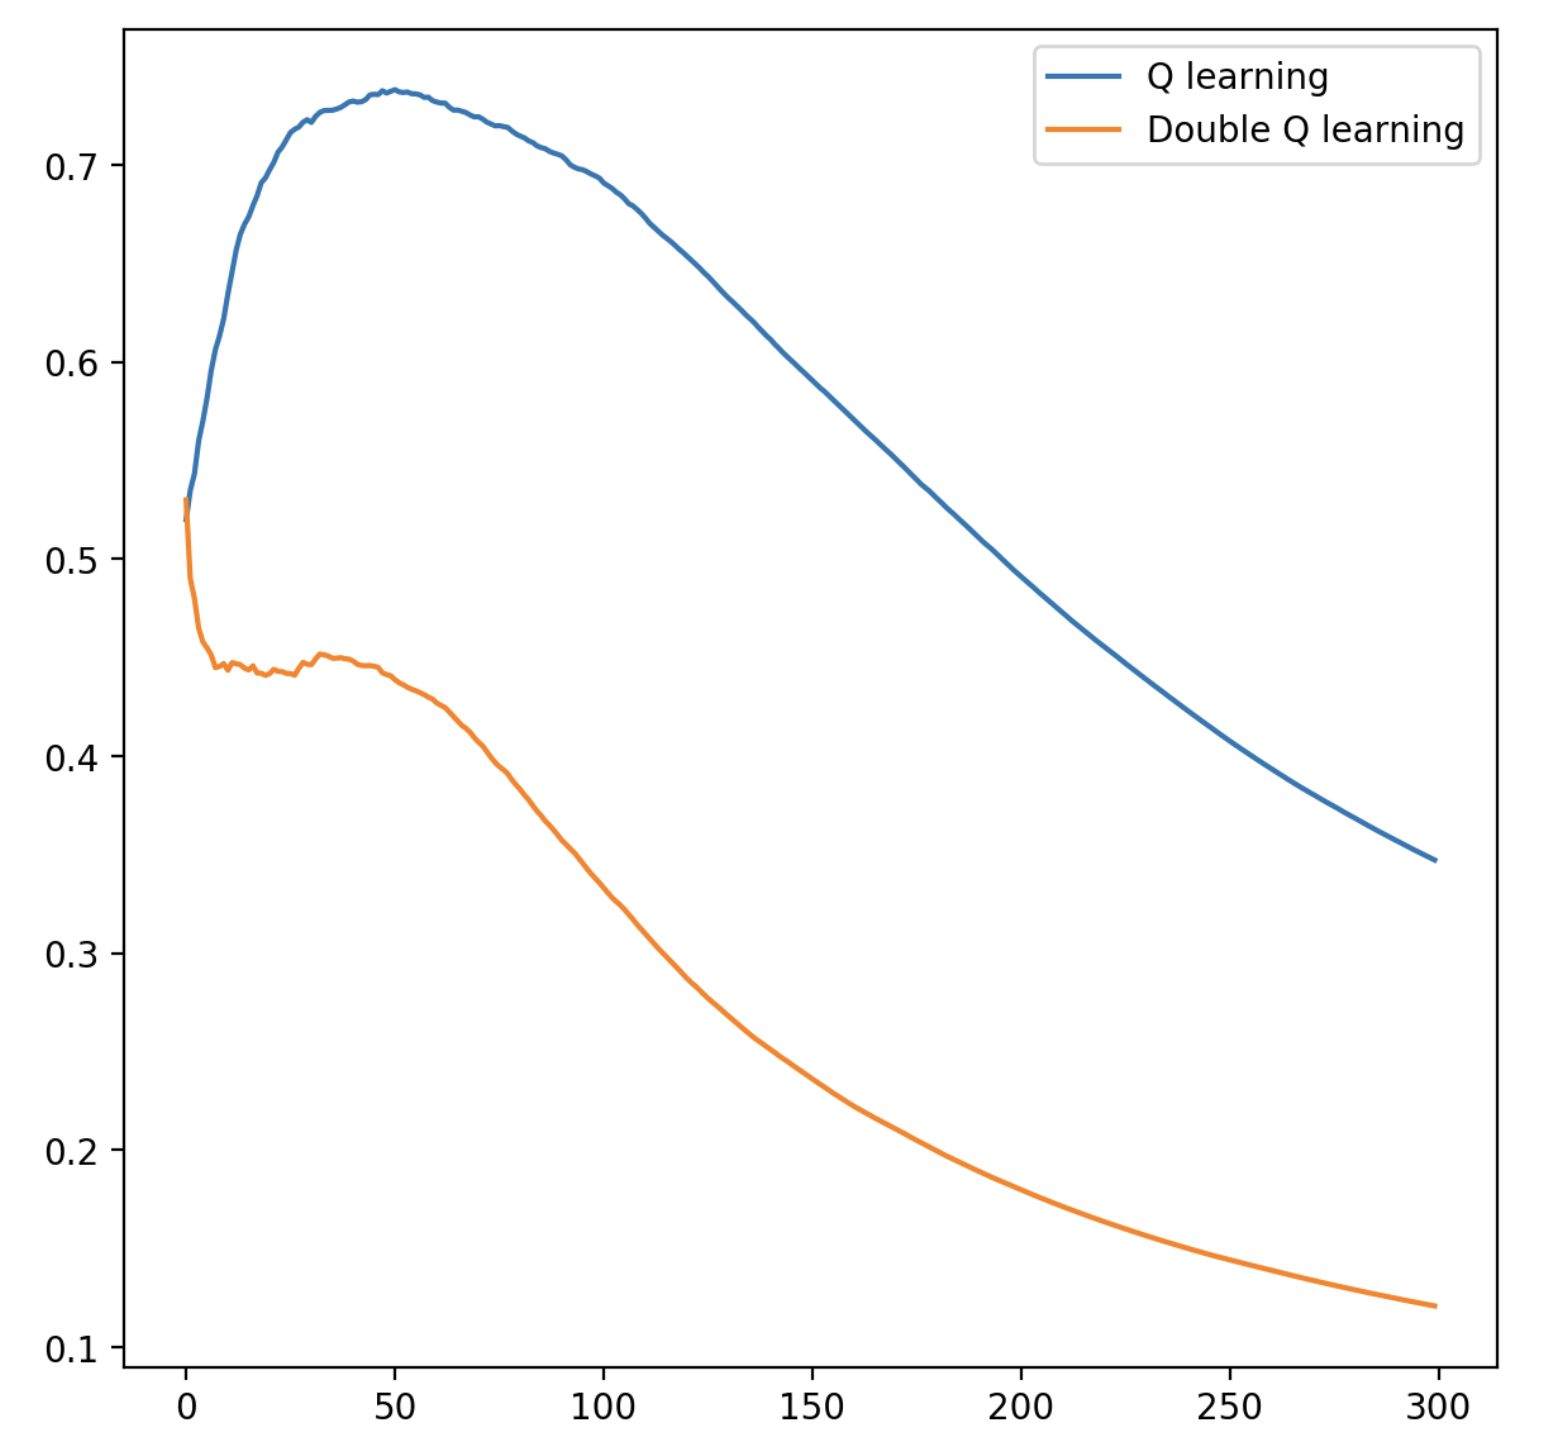
\includegraphics[width=0.7\linewidth]{pic/doubleQ.png}
    \caption{Ratio of selecting the wrong actions.}
\end{figure}
\end{frame}


% \begin{frame}{Cooperative v.s. Self-interested}

% \begin{exampleblock}{Cooperative agents:}
% \begin{itemize}
%     \item Input: {a weighted graph, N agents (starts/goals)}
    
%     \item Objective: {minimize global cost}
% \end{itemize}
% \end{exampleblock}

% \pause
% \begin{exampleblock}{Self-interested agents:}
% \begin{itemize}
%     \item Objective: {minimize \textbf{individual cost}}

%     \pause
%     \item A naïve way: {each schedule herself individually, resolve conflicts randomly}
% \end{itemize}
% \end{exampleblock}

% \end{frame}


% \begin{frame}{Relation with Traffic Control}

% \begin{exampleblock}{Traffic flow network:}
% \begin{itemize}
%     \item Continuous flow along edges, causing certain \alert{delays}

%     \item Selfish routing is proved to be non-optimal

%     \item Toll/taxation mechanisms are usaully used.

%     \item Sometimes coincides with congestion games (a classical \alert{potential game}) 
% \end{itemize}
% \end{exampleblock}

% \end{frame}



% \begin{frame}{An Example}

% % \begin{figure}[htpb]
% %         \centering
% %         \includegraphics[width=0.6\linewidth]{pic/tax_eg.png}
% % \end{figure}

% \begin{columns}
%     \begin{column}{.5\textwidth}
%     \centering
%         \underline{Selfish routing} \\
%         a1: \{S1, \_, C, G1\} \\
%         a2: \{S2, C, G2\} \\
%         a3: \{S3, \_, C, G3\} \\
%         $\Rightarrow (3+\alert{1}) + 2 + (3+\alert{2}) = 11$
%     \end{column}    

%     \pause
%     \begin{column}{.5\textwidth}
%     \centering
%         \underline{With taxation} \\
%         a1: \{S1, left-hand, G1\} \\
%         a2: \{S2, C, G2\} \\
%         a3: \{S3, right-hand, G3\} \\
%         $\Rightarrow \alert{4} + 2 + \alert{4} = 10$
%     \end{column}
% \end{columns}

% \end{frame}


% \begin{frame}{Formally}

% \begin{exampleblock}{Key idea:}
% \begin{itemize}
%     \item Assign each edge/vertex a tax (penalty)

%     \item Individually minimizes $\hat{c}(P_i) = c(P_i) + T(P_i)$

%     \pause[2]
%     \item \alert{$\Rightarrow$ Iterative Taxation Framework}
%     % \begin{figure}[htpb]
%     %     \centering
%     %     \includegraphics[width=0.8\linewidth]{pic/ITF.png}
%     % \end{figure}

%     \pause[3]
%     \item Implementations: 1) Exhaustive 2) Monte-Carlo
% \end{itemize}
% \end{exampleblock}

% \end{frame}


% \begin{frame}{Evaluation -- toy example}

% % \begin{figure}[htpb]
% %         \centering
% %         \includegraphics[width=1\linewidth]{pic/result_3x3.png}
% %         \caption{EITA (exhaustive iterative taxation algorithm),
% %                 MC-ITA (Monte-Carlo iterative taxation algorithm),
% %                 Lowerbound (global optimum)} 
% % \end{figure}

% \end{frame}


% \begin{frame}{Evaluation -- large scale}

% \begin{columns}
%     \begin{column}{.65\columnwidth}
%         % \begin{figure}[htpb]
%         %     \centering
%         %     \includegraphics[width=1\linewidth]{pic/result_den520.png}
%         %     \caption{den520d for 10 agents}
%         % \end{figure}
%     \end{column}

%     \begin{column}{.35\columnwidth}
%         % \begin{figure}[htpb]
%         %     \centering
%         %     \includegraphics[width=1\linewidth]{pic/den520d.pdf}
%         %     \caption{den520d -- dimension ($257\times 256$), \#states (28178)}
%         % \end{figure}
%     \end{column}
% \end{columns}

% \end{frame}


% \begin{frame}{Drawbacks}

% \begin{itemize}
%     \item Not guaranteed to minimize global cost (maximize social welfare)

%     \item Not strategyproof: agents could misreport their starts/goals

%     \item Agents are restricted to be homogeneous

%     \pause
%     \item \alert{Let's seek help from auctions!}
% \end{itemize}

% \end{frame}



% \begin{frame}{Conventional Combinatorial Auction}

% \begin{exampleblock}{Preliminaries}
%     \begin{itemize}
%         \item Agents: $N = \{1, \cdots, n\}$

%         \item Actioned items: $M = \{1, \cdots, m\}$

%         \item Valuation function for each agent $v_i: 2^M \mapsto \mathbb{R}$

%         \pause
%         \alert{
%         \item A mechanism (with monetary transfer) is a pair of
%         \begin{itemize}
%             \item a social choice function $f: V_1 \times \cdots \times V_n \mapsto A$
            
%             \item a vector of payments functions $p_1, \cdots, p_n$, where $p_i: V_1 \times \cdots \times V_n \mapsto \mathbb{R}$
%         \end{itemize}}
%     \end{itemize}
% \end{exampleblock}

% \end{frame}


% \begin{frame}{Reduce to CA}

%     % \begin{figure}[htpb]
%     %     \centering
%     %     \includegraphics[width=1\linewidth]{pic/reduction.png}
%     % \end{figure}

%     \pause
%     \begin{exampleblock}{Derived valuation function:}
%     \begin{itemize}[<+-| alert@+>]
%         \item $v_i(p) = val(g_i) - c(p)$

%         \item Turns out $val(g_i) := max_c \times n$ [constant]
%     \end{itemize}
%     \end{exampleblock}

% \end{frame}


% \begin{frame}{Strategic Manipulation}

%     % \begin{figure}[htpb]
%     %     \centering
%     %     \includegraphics[width=0.4\linewidth]{pic/ca_eg.png}
%     %     \caption{Assuming $v_i(g_i) = 10$}
%     % \end{figure}

%     \begin{exampleblock}{A centralized yet not strategyproof mechanism:}
%     \begin{itemize}[<+-| alert@+>]
%         \item If a1 and a2 report truthfully,
%             \begin{itemize}
%                 \item a1 gets 10-(1.5+1), a2 gets 10-(1+1)
%             \end{itemize}

%         \item If a1 misreports (s1, X) = 1.8,
%             \begin{itemize}
%                 \item a1 gets 10-(1+1), a2 gets 10-(1.7+1)
%             \end{itemize}
%     \end{itemize}
%     \end{exampleblock}

% \end{frame}


% \begin{frame}{Strategic Manipulation}

%     % \begin{figure}[htpb]
%     %     \centering
%     %     \includegraphics[width=0.3\linewidth]{pic/ca_eg.png}
%     %     \caption{Assuming $v_i(g_i) = 10$}
%     % \end{figure}

%     \begin{exampleblock}{The well-known VCG mechanism:}
%     \begin{itemize}[<+-| alert@+>]
%         \item Payment := the harm you did to others' social welfare

%         \item If a1 and a2 report truthfully,
%             \begin{itemize}
%                 \item a1 gets 10-(1.5+1)-0 = 7.5, a2 gets 10-(1+1)-0.5
%             \end{itemize}

%         \item If a1 misreports (s1, X) = 1.8,
%             \begin{itemize}
%                 \item a1 gets 10-(1+1)-0.7 = 7.3, a2 gets 10-(1.7+1)-0
%             \end{itemize}
%     \end{itemize}
%     \end{exampleblock}

% \end{frame}


% \begin{frame}{Computational Issues}

% \begin{itemize}
%     \item In sealed-bid auctions, such as VCG, each agent needs to bid over all bundles that it may be interested in. 

%     \item In MAPF, this means that an agent $i$ would need to find all paths from $s_i$ to $g_i$ and place bids on them.

%     \item The number of paths between two vertices in a graph may be exponential in the path length.

%     \item Moreover, to find an allocation that maximizes its revenue, the auctioneer will need to check the cross product of these potentially exponential number of bids.

%     \pause
%     \item \alert{Interative combinatorial auction (Parkes 2006)}
% \end{itemize}

% \end{frame}


% \begin{frame}{Iterative Combinatorial Auction}

% \begin{exampleblock}{Basic framework (\textit{iBundle}):}
% \begin{itemize}
%     \item Bidding

%     \item Winner determination

%     \item Price update
% \end{itemize}
% \end{exampleblock}

% \end{frame}


% \begin{frame}{iBundle -- Bidding}

%     % \begin{figure}[htpb]
%     %     \centering
%     %     \includegraphics[width=0.8\linewidth]{pic/bidding.png}
%     % \end{figure}

%     \begin{exampleblock}{Bidding:}
%         \begin{itemize}[<+-| alert@+>]
%             \item Agents place \texttt{XOR} bids on their \underline{desired} bundles.

%             \item Minimize $cost(p) + ask(p)$

%             \item $a_3$ bids $[<F, t_1>, <D, t_2>, <G, t_3>, <E, t_4>, <I, t_5>]; [<F, t_1>, <D, t_2>, <C, t_3>, <E, t_4>, <I, t_5>]$.

%             \item Myopic best response is a dominant strategy
%         \end{itemize}
%     \end{exampleblock}

% \end{frame}


% \begin{frame}{iBundle -- Winner Dermination}

%     % \begin{figure}[htpb]
%     %     \centering
%     %     \includegraphics[width=0.8\linewidth]{pic/bidding.png}
%     % \end{figure}

%     \begin{exampleblock}{Winner determination:}
%         \begin{itemize}[<+-| alert@+>]
%             \item Determine a provisional allocation

%             \item To maximizes seller's revenue and include more non-conflicting agents

%             \item $a_1$ gets $[<A, t_1>, <C, t_2>]$, $a_3$ gets $[<F, t_1>, <D, t_2>, <G, t_3>, <E, t_4>, <I, t_5>]$
%         \end{itemize}
%     \end{exampleblock}

% \end{frame}


% \begin{frame}{iBundle -- Price Update}

%     % \begin{figure}[htpb]
%     %     \centering
%     %     \includegraphics[width=0.8\linewidth]{pic/bidding.png}
%     % \end{figure}

%     \begin{exampleblock}{Price update:}
%         \begin{itemize}[<+-| alert@+>]
%             \item Initial prices for all bundles are 0

%             \item Bundles that ``unhappy'' agents bid on are raised by $\epsilon$

%             \item In MAPF, sufficient to set $\epsilon = \min(c_e)$

%             \item $a_2$ is unhappy, prices of paths of $MDD_2^3$ are raised by 1
%         \end{itemize}
%     \end{exampleblock}

% \end{frame}


% \begin{frame}{Evaluation}
%     % \begin{figure}[htpb]
%     %     \includegraphics[width=0.6\linewidth]{pic/ca_small}
%     % \end{figure}
% \end{frame}


% \begin{frame}{Evaluation}
%     % \begin{figure}[htpb]
%     %     \includegraphics[width=0.6\linewidth]{pic/ca_large}
%     % \end{figure}
% \end{frame}



% %%%%%%%%%% part 4 %%%%%%%%%%


% \begin{frame}{Insights}

% \begin{itemize}[<+-| alert@+>]
%     \item Consider heterogeneous and self-interested agents

%     \item Still, complexity issues due to the combinatorial nature

%     \item One-parameter agents, e.g. fuel consumption  
%     \begin{itemize}
%         \item Seems poly-time strategyproof mechanism exists \cite{machida2019polynomial}
%     \end{itemize}

%     \item Negotiation and bargaining on paths\cite{inotsume2020path}
% \end{itemize}

% \end{frame}


% \begin{frame}[allowframebreaks]
%     \bibliography{ref}
%     \bibliographystyle{alpha}
%     % If too many references, use this command to resize:
%     % \tiny\bibliographystyle{alpha}
% \end{frame}


\begin{frame}
    \begin{center}
        {\Huge\calligra Thanks!}
    \end{center}
\end{frame}


% \begin{frame}{A Running Example}
    % \begin{figure}[htpb]
    %     \centering
    %     \includegraphics[width=0.5\linewidth]{pic/mapf_ca_eg.png}
        
    %     \pause
    %     \includegraphics[width=1\linewidth]{pic/mapf_ca_proc_1.png}
        
    %     \pause
    %     \includegraphics[width=1\linewidth]{pic/mapf_ca_proc_2.png}
        
    %     \pause
    %     \includegraphics[width=1\linewidth]{pic/mapf_ca_proc_3.png}
    % \end{figure}
% \end{frame}

% \begin{frame}{Sequential $\to$ Decentralized}
%     \begin{block}{}
%         \begin{figure}[htpb]
%             \centering
%             \includegraphics[width=0.3\linewidth]{pic/gradient.png}
%         \end{figure}
%     \end{block}

%     \pause
%     \begin{columns}
%         \begin{column}{.5\textwidth}
%         \centering
%             \begin{exampleblock}{Sequential update}
%                 \begin{itemize}
%                     \item
%                     For $i = 1 \to k$,
%                     \begin{itemize}
%                         \item While not converge,
%                         \begin{itemize}
%                             \item \texttt{Gradient ascent}
%                         \end{itemize}
%                     \end{itemize}
%                 \end{itemize}
%             \end{exampleblock}
%         \end{column}    

%         \pause
%         \begin{column}{.5\textwidth}
%         \centering
%             \begin{exampleblock}{Decentralized update}
%                 \begin{itemize}
%                     \item
%                     For every $i \in [1..k]$,
%                     \begin{itemize}
%                         \item While not converge,
%                         \begin{itemize}
%                             \item \texttt{Gradient ascent}
%                             \item \alert{\texttt{Broadcast}$({v}_i)$}
%                         \end{itemize}
%                     \end{itemize}
%                 \end{itemize}
%             \end{exampleblock}
%         \end{column}
%     \end{columns}
% \end{frame}


% \begin{frame}{Issues}
%     \begin{columns}
%         \begin{column}{.3\columnwidth}
%             \begin{figure}[htpb]
%                 \centering
%                 \includegraphics[width=1.1\linewidth]{pic/bias.png}
%             \end{figure}
%         \end{column}

%         \begin{column}{.7\columnwidth}
%             \begin{itemize}[<+-| alert@+>]
%                 \item 
%                 MNIST for minibatch sizes of 1024 (top), 512 (middle), and 256 (bottom)

%                 \item
%                 The figure shows the performance of EigenGame degrades in the low batch size regime.

%                 % \item
%                 % Because we use the same minibatch for all inner products in the gradient which contains products and ratios of random variables.

%                 \item Current hardware easily supports batches of 1024 for MNIST and 128 for IMAGENET

%                 \item \underline{\textbf{But still, can we reduce the bias?}}
%             \end{itemize}
%         \end{column}
%     \end{columns}
% \end{frame}


% \begin{frame}{Figure and Column}
%     % From thuthesis user guide.
%     \begin{minipage}[c]{0.3\linewidth}
%     %%% DO NOT USE PSTricks in pdflatex
% %         \psset{unit=0.8cm}
% %         \begin{pspicture}(-1.75,-3)(3.25,4)
% %             \psline[linewidth=0.25pt](0,0)(0,4)
% %             \rput[tl]{0}(0.2,2){$\vec e_z$}
% %             \rput[tr]{0}(-0.9,1.4){$\vec e$}
% %             \rput[tl]{0}(2.8,-1.1){$\vec C_{ptm{ext}}$}
% %             \rput[br]{0}(-0.3,2.1){$\theta$}
% %             \rput{25}(0,0){%
% %             \psframe[fillstyle=solid,fillcolor=lightgray,linewidth=.8pt](-0.1,-3.2)(0.1,0)}
% %             \rput{25}(0,0){%
% %             \psellipse[fillstyle=solid,fillcolor=yellow,linewidth=3pt](0,0)(1.5,0.5)}
% %             \rput{25}(0,0){%
% %             \psframe[fillstyle=solid,fillcolor=lightgray,linewidth=.8pt](-0.1,0)(0.1,3.2)}
% %             \rput{25}(0,0){\psline[linecolor=red,linewidth=1.5pt]{->}(0,0)(0.,2)}
% % %           \psRotation{0}(0,3.5){$\dot\phi$}
% % %           \psRotation{25}(-1.2,2.6){$\dot\psi$}
% %             \psline[linecolor=red,linewidth=1.25pt]{->}(0,0)(0,2)
% %             \psline[linecolor=red,linewidth=1.25pt]{->}(0,0)(3,-1)
% %             \psline[linecolor=red,linewidth=1.25pt]{->}(0,0)(2.85,-0.95)
% %             \psarc{->}{2.1}{90}{112.5}
% %             \rput[bl](.1,.01){C}
% %         \end{pspicture}
%     \end{minipage}\hspace{1cm}
%     \begin{minipage}{0.5\linewidth}
%         \medskip
%         %\hspace{2cm}
%         \begin{figure}[h]
%             \centering
%             \includegraphics[height=.4\textheight]{pic/dtmf.pdf}
%         \end{figure}
%     \end{minipage}
% \end{frame}

% \begin{frame}[fragile]{\LaTeX{} Commands}
%     \begin{exampleblock}{Commands}
%         \centering
%         \footnotesize
%         \begin{tabular}{llll}
%             \cmd{chapter} & \cmd{section} & \cmd{subsection} & \cmd{paragraph} \\
%             Chapter & Section & Subsection & Paragraph \\\hline
%             \cmd{centering} & \cmd{emph} & \cmd{verb} & \cmd{url} \\
%             Centre Align & Emphasis & Verbatim & Hyperlink \\\hline
%             \cmd{footnote} & \cmd{item} & \cmd{caption} & \cmd{includegraphics} \\
%             Foodnote & Item & Caption & FigP\&Pic \\\hline
%             \cmd{label} & \cmd{cite} & \cmd{ref} \\
%             Label & Citing & Referring\\\hline
%         \end{tabular}
%     \end{exampleblock}
%     \begin{exampleblock}{Environment Command}
%         \centering
%         \footnotesize
%         \begin{tabular}{lll}
%             \env{table} & \env{figure} & \env{equation}\\
%             Table & Figure & Equation \\\hline
%             \env{itemize} & \env{enumerate} & \env{description}\\
%             Bullets & Numbering & Description \\\hline
%         \end{tabular}
%     \end{exampleblock}
% \end{frame}

% \begin{frame}[fragile]{\LaTeX{} Environment Command Samples}
%     \begin{minipage}{0.5\linewidth}
% \begin{lstlisting}[language=TeX]
% \begin{itemize}
%   \item A \item B
%   \item C
%   \begin{itemize}
%     \item C-1
%   \end{itemize}
% \end{itemize}
% \end{lstlisting}
%     \end{minipage}\hspace{1cm}
%     \begin{minipage}{0.3\linewidth}
%         \begin{itemize}
%             \item A
%             \item B
%             \item C
%             \begin{itemize}
%                 \item C-1
%             \end{itemize}
%         \end{itemize}
%     \end{minipage}
%     \medskip
%     \pause
%     \begin{minipage}{0.5\linewidth}
% \begin{lstlisting}[language=TeX]
% \begin{enumerate}
%   \item Class 1 
%   \item Class 2
%   \item Class 2
%   \begin{itemize}
%     \item[n+e] Student 1
%   \end{itemize}
% \end{enumerate}
% \end{lstlisting}
%     \end{minipage}\hspace{1cm}
%     \begin{minipage}{0.3\linewidth}
%         \begin{enumerate}
%             \item Class 1
%             \item Class 2
%             \item Class 3
%             \begin{itemize}
%                 \item[n+e] Student 1
%             \end{itemize}
%         \end{enumerate}
%     \end{minipage}
% \end{frame}

% \begin{frame}[fragile]{\LaTeX{} Equations}
%     \begin{columns}
%         \begin{column}{.55\textwidth}
% \begin{lstlisting}[language=TeX]
% $V = \frac{4}{3}\pi r^3$

% \[
%   V = \frac{4}{3}\pi r^3
% \]

% \begin{equation}
%   \label{eq:vsphere}
%   V = \frac{4}{3}\pi r^3
% \end{equation}
% \end{lstlisting}
%         \end{column}
%         \begin{column}{.4\textwidth}
%             $V = \frac{4}{3}\pi r^3$
%             \[
%                 V = \frac{4}{3}\pi r^3
%             \]
%             \begin{equation}
%                 \label{eq:vsphere}
%                 V = \frac{4}{3}\pi r^3
%             \end{equation}
%         \end{column}
%     \end{columns}
%     \begin{itemize}
%         \item Check more \href{https://en.wikipedia.org/wiki/Help:Displaying_a_formula}{\color{purple}{Here}}
%     \end{itemize}
% \end{frame}

% \begin{frame}[fragile]
%     \begin{columns}
%         \column{.6\textwidth}
% \begin{lstlisting}[language=TeX]
% \begin{table}[htbp]
%   \caption{Definition}
%   \label{tab:number}
%   \centering
%   \begin{tabular}{cl}
%     \toprule
%     Word & Definition \\
%     \midrule
%     1 & 4.0 \\
%     2 & 3.7 \\
%     \bottomrule
%   \end{tabular}
% \end{table}
% Check definition of 
% Equation~(\ref{eq:vsphere}) 
% in Table~\ref{tab:number}。
% \end{lstlisting}
%         \column{.4\textwidth}
%         \begin{table}[htpb]
%             \centering
%             \caption{Definition}
%             \label{tab:number}
%             \begin{tabular}{cl}\toprule
%                 Eq. & Def. \\\midrule
%                 1 & 4.0\\
%                 2 & 3.7\\\bottomrule
%             \end{tabular}
%         \end{table}
%         \normalsize Please check the definition of Equation~(\ref{eq:vsphere}) in Table~\ref{tab:number}
%     \end{columns}
% \end{frame}

% \begin{frame}{Plotting}
%     \begin{itemize}
%         \item Vector: eps, ps, pdf
%         \begin{itemize}
%             \item METAPOST, pstricks, pgf $\ldots$
%             \item Xfig, Dia, Visio, Inkscape $\ldots$
%             \item Export Matlab / Excel as pdf
%         \end{itemize}
%         \item Bitmap: png, jpg, tiff $\ldots$
%         \begin{itemize}
%             \item Avoiding using bitmaps 
%         \end{itemize}
%     \end{itemize}
%     \begin{figure}[htpb]
%         \centering
%         \includegraphics[width=0.2\linewidth]{pic/QUT_Logo_CMYK.jpg}
%         \caption{This is a Bitmaps}
%     \end{figure}
% \end{frame}

\end{document}